\documentclass{article}

\usepackage{amsmath, amsthm, amssymb}
\usepackage{geometry}
\geometry{a4paper, top=25mm, left=10mm, right=10mm, bottom=30mm,
headsep=10mm, footskip=12mm}
\usepackage{graphicx}
\usepackage{lscape}
\begin{document} 

\begin{landscape}
\section{linear BSplines}
\subsection{Functions}\begin{eqnarray*} \varphi_1 & = & \begin{array}{cc}
 \{ & 
\begin{array}{cc}
 3.464101615137754587054892683011744733886-3.464101615137754587054892683011744733886 x & x\geq \frac{1}{2}\land x<1 \\
 3.464101615137754587054892683011744733886 x & x\geq 0\land x<\frac{1}{2}
\end{array}

\end{array}\\
\varphi_2 & = & \begin{array}{cc}
 \{ & 
\begin{array}{cc}
 5.899238271937257294501362767049163407493-14.13397337635908350175125253003286143671 x & x\geq \frac{1}{4}\land x<\frac{1}{2} \\
 9.462979711389945676254198538163792193264 x & x\geq 0\land x<\frac{1}{4} \\
 1.677990269774715967092441885048676787527 x-1.677990269774715967092441885048676787527 & x\geq \frac{3}{4}\land x<1 \\
 2.993003395194421858404612106820392455916 x-2.664250113839495385576569551377463538819 & x\geq \frac{1}{2}\land x<\frac{3}{4}
\end{array}

\end{array}\\
\varphi_3 & = & \begin{array}{cc}
 \{ & 
\begin{array}{cc}
 2.171240593367237661666963458005663576797-11.00419101450331474148978598108946236703 x & x\geq 0\land x<\frac{1}{4} \\
 2.900385249116278975073458711553274065599 x-1.304903472537660767473847715155020531360 & x\geq \frac{1}{4}\land x<\frac{1}{2} \\
 5.926963045931216321639528986349047536287 x+2.226035845481337351211347364005908109395 & x\geq -\frac{1}{2}\land x<-\frac{1}{4} \\
 5.707782037474817563461993362348069405897 x+2.171240593367237661666963458005663576797 & x\geq -\frac{1}{4}\land x<0 \\
 0.4842971734015957335429388020720550048003-0.6780160427622340269601143229008770067205 x & x\geq \frac{1}{2}\land x<\frac{3}{4} \\
 0.09685943468031914670858776041441100096007 x-0.09685943468031914670858776041441100096007 & x\geq \frac{3}{4}\land x<1 \\
 0.4916304516561805397389447527790771058323 x+0.4916304516561805397389447527790771058323 & x\geq -1\land x<-\frac{3}{4} \\
 -3.441413161593263778172613269453539740826 x-2.458152258280902698694723763895385529162 & x\geq -\frac{3}{4}\land x<-\frac{1}{2}
\end{array}

\end{array}\end{eqnarray*}
\end{landscape}
\begin{landscape}
\subsection{Graphics}
\begin{tabular}{ccc}
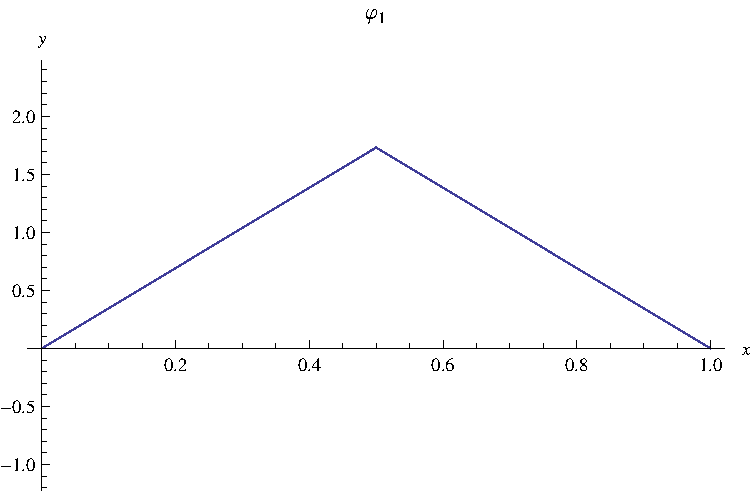
\includegraphics[width=6.7cm]{linear_bspline_1.pdf}& 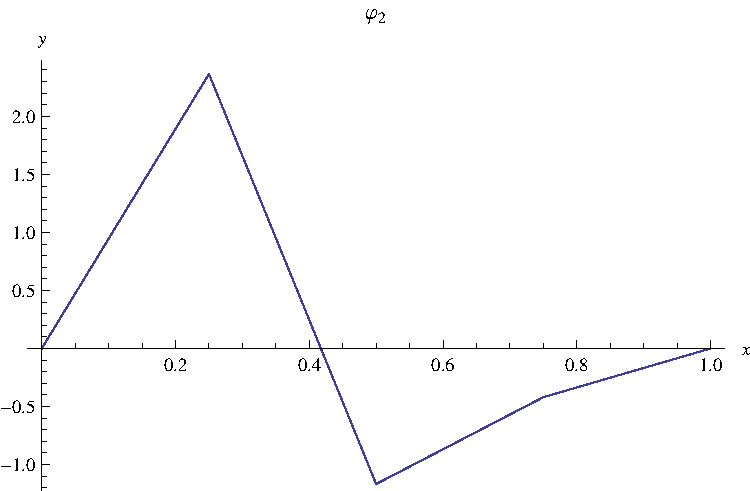
\includegraphics[width=6.7cm]{linear_bspline_2.pdf}& 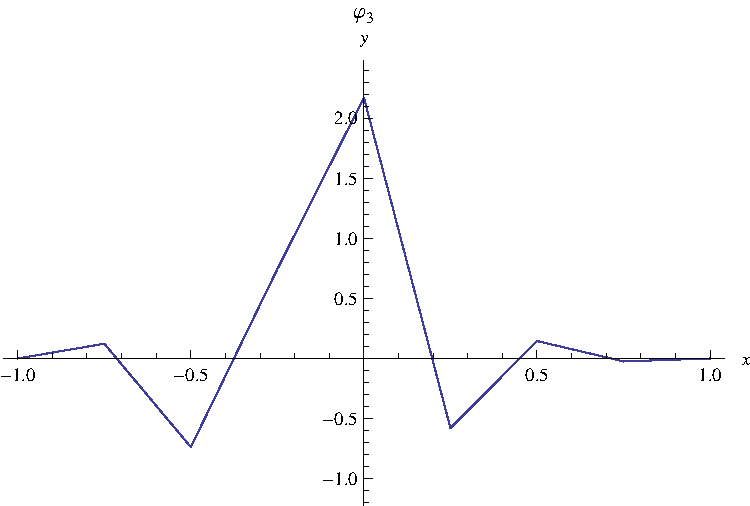
\includegraphics[width=6.7cm]{linear_bspline_3.pdf} \\
\end{tabular} 
 \end{landscape}
 \begin{landscape}
 \subsection{Validation}$$ \begin{array}{l|lll}
\int_{-1}^1 f_1(x)f_2(x) dx& \varphi_1(x)& \varphi_2(x)& \varphi_3(x) \\ \hline 
 \varphi_1(x) & 1.0000 & 0.\cdot 10^{(-397)} & 0.\cdot 10^{(-388)} \\ 
\varphi_2(x) & 0.\cdot 10^{(-397)} & 1.0000 & 0.\cdot 10^{(-388)} \\ 
\varphi_3(x) & 0.\cdot 10^{(-388)} & 0.\cdot 10^{(-388)} & 1.0000 \\ 
\end{array} $$
$$ \begin{array}{l|lll}
\int_{-1}^1 f_1(x)f_2(x-1) dx& \varphi_1(x-1)& \varphi_2(x-1)& \varphi_3(x-1) \\ \hline 
 \varphi_1(x) & 0 & 0 & 0.\cdot 10^{(-387)} \\ 
\varphi_2(x) & 0 & 0 & 0.\cdot 10^{(-387)} \\ 
\varphi_3(x) & 0 & 0 & 3.56428\cdot 10^{(-291)} \\ 
\end{array} $$ 
\end{landscape} 
 \begin{landscape}
 \subsection{linear BSpline dirichlet boundary Functions}
 \begin{eqnarray*}
 \\ 
\end{eqnarray*}
\end{landscape}
\begin{landscape}
\subsection{BSpline Dirichlet boundary Graphics}
\begin{tabular}{}
\end{tabular} 
 \\ 
\begin{tabular}{}
\end{tabular} 
 \end{landscape}
 \begin{landscape}
 \subsection{Validation}\end{landscape} 
 \begin{landscape}
\section{Wavelets}
\subsection{Functions}
 \begin{eqnarray*}
\Psi_1 & = & \begin{array}{cc}
 \{ & 
\begin{array}{cc}
 9.723126539105882521464898595634958934608 x-3.007148855493370156848660634030297053580 & x\geq \frac{1}{4}\land x<\frac{3}{8} \\
 9.403364908845459223390544479169305803909 x-2.887238244145711420070777840355677129568 & x\geq \frac{3}{8}\land x<\frac{1}{2} \\
 0.5634759370212272862047463938812607934943 x & x\geq 0\land x<\frac{1}{8} \\
 0.7172362049722063480336225835918725183016-5.174413702756423498064234274853719352919 x & x\geq \frac{1}{8}\land x<\frac{1}{4} \\
 22.32888385765284908917219560533931950206-41.02887929475166179509540241222068745935 x & x\geq \frac{1}{2}\land x<\frac{5}{8} \\
 35.21839390402398429095779425659595183891 x-25.32566189158192971461105231267108005935 & x\geq \frac{5}{8}\land x<\frac{3}{4} \\
 5.945952234421770538030196839347160288883-6.477091597314282712563871279428368625401 x & x\geq \frac{3}{4}\land x<\frac{7}{8} \\
 2.227976694174185316294475758778701933254-2.227976694174185316294475758778701933254 x & x\geq \frac{7}{8}\land x<1
\end{array}

\end{array}\\
\Psi_2 & = & \begin{array}{cc}
 \{ & 
\begin{array}{cc}
 8.381465920375111721923549460260546989328 x-3.523179956205757665732383336706792239211 & x\geq \frac{1}{4}\land x<\frac{3}{8} \\
 5.329795045029748543732045947467489821543 x-2.378803377951246473910569519409395801292 & x\geq \frac{3}{8}\land x<\frac{1}{2} \\
 21.66875207906325351789286612920801076590 x & x\geq 0\land x<\frac{1}{8} \\
 6.845001495877793114724712503943658183355-33.09125988795909139990483390234125470094 x & x\geq \frac{1}{8}\land x<\frac{1}{4} \\
 0.9536471485454259931848448477478303649327-1.335106007963596390458782786846962510906 x & \left(x\geq \frac{1}{2}\land x<\frac{5}{8}\right)\lor \left(x\geq \frac{5}{8}\land x<\frac{3}{4}\right) \\
 0.1907294297090851986369689695495660729865 x-0.1907294297090851986369689695495660729865 & \left(x\geq \frac{3}{4}\land x<\frac{7}{8}\right)\lor \left(x\geq \frac{7}{8}\land x<1\right) \\
 -5.021188345105564723209857021939489980700 x-1.761589978102878832866191668353396119605 & x\geq -\frac{1}{2}\land x<-\frac{3}{8} \\
 -13.01056641923786902975638334318054460197 x-4.757606755902492947821139038818791602583 & x\geq -\frac{3}{8}\land x<-\frac{1}{4} \\
 6.242476994555099014474397381405268547587 x+0.05565409754574906323655614232766168480683 & x\geq -\frac{1}{4}\land x<-\frac{1}{8} \\
 5.797244214189106508581948242783975069132 x & x\geq -\frac{1}{8}\land x<0 \\
 -0.4993361296332690191591578950775659138297 x-0.4993361296332690191591578950775659138297 & x\geq -1\land x<-\frac{3}{4} \\
 3.495352907432883134114105265542961396808 x+2.496680648166345095795789475387829569148 & x\geq -\frac{3}{4}\land x<-\frac{1}{2}
\end{array}

\end{array}\\
\Psi_3 & = & \begin{array}{cc}
 \{ & 
\begin{array}{cc}
 2.171240593367237661666963458005663576797-33.01257304350994422446935794326838710109 x & x\geq 0\land x<\frac{1}{8} \\
 22.60573201096843064178362082730255862943 x-4.781047538442559196614658888315704639517 & x\geq \frac{1}{8}\land x<\frac{1}{4} \\
 18.00007014625004772309612258304812073925 x+2.280831097595437040755731270006152641992 & x\geq -\frac{1}{4}\land x<-\frac{1}{8} \\
 17.12334611242445269038598008704420821769 x+2.171240593367237661666963458005663576797 & x\geq -\frac{1}{8}\land x<0 \\
 2.273497819340852234559725319299130540960-5.612449420165215082913916003156782092481 x & x\geq \frac{1}{4}\land x<\frac{3}{8} \\
 1.111184603177022474056672194326198529439-2.512947510395002388239107669895630061759 x & x\geq \frac{3}{8}\land x<\frac{1}{2} \\
 -3.960441239306494162683749975232739112957 x-1.242774942168976271733457858447753897730 & x\geq -\frac{1}{2}\land x<-\frac{3}{8} \\
 -19.69261569230427143432998206416320649959 x-7.142340362043142748600794891796679167718 & x\geq -\frac{3}{8}\land x<-\frac{1}{4} \\
 0.6780160427622340269601143229008770067205 x-0.4842971734015957335429388020720550048003 & x\geq \frac{1}{2}\land x<\frac{3}{4} \\
 0.09685943468031914670858776041441100096007-0.09685943468031914670858776041441100096007 x & x\geq \frac{3}{4}\land x<1 \\
 -0.4916304516561805397389447527790771058323 x-0.4916304516561805397389447527790771058323 & x\geq -1\land x<-\frac{3}{4} \\
 3.441413161593263778172613269453539740826 x+2.458152258280902698694723763895385529162 & x\geq -\frac{3}{4}\land x<-\frac{1}{2}
\end{array}

\end{array}\end{eqnarray*}
\end{landscape}
\begin{landscape}
\subsection{Graphics}
\begin{tabular}{ccc}
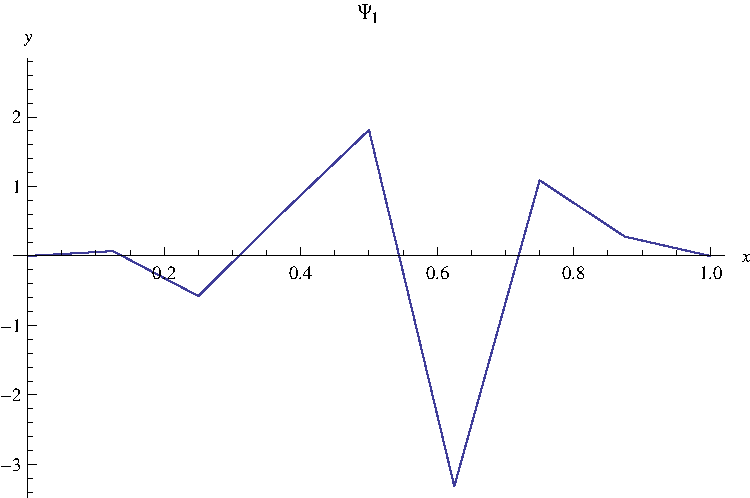
\includegraphics[width=6.7cm]{linear_wavelet_1.pdf}& 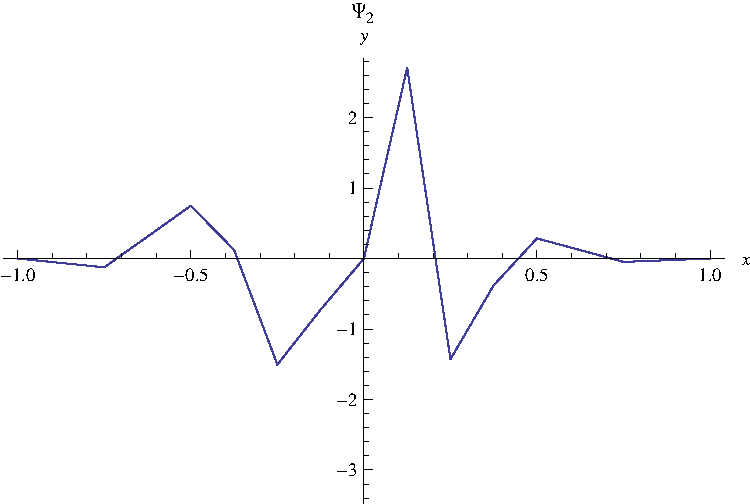
\includegraphics[width=6.7cm]{linear_wavelet_2.pdf}& 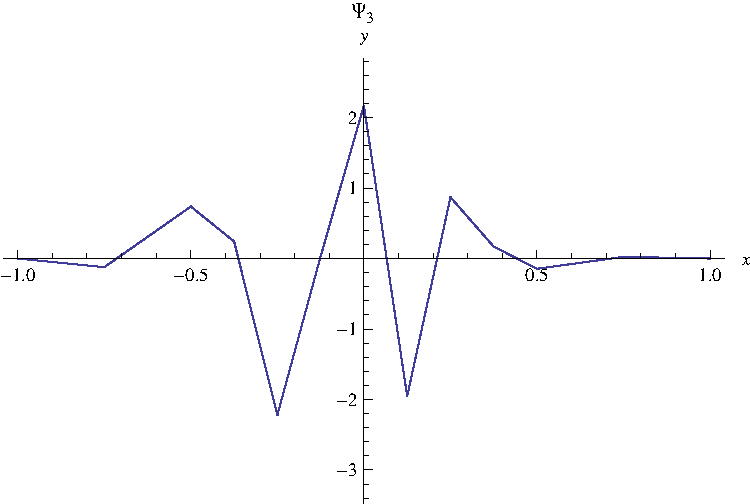
\includegraphics[width=6.7cm]{linear_wavelet_3.pdf} \\
\end{tabular} 
 \end{landscape}
 \begin{landscape}
 \subsection{Validation}$$ \begin{array}{l|lll}
\int_{-1}^1 f_1(x)f_2(x) dx& \Psi_1(x)& \Psi_2(x)& \Psi_3(x) \\ \hline 
 \Psi_1(x) & 1.0000 & 1.51263\cdot 10^{(-291)} & 2.97857\cdot 10^{(-291)} \\ 
\Psi_2(x) & 1.51263\cdot 10^{(-291)} & 1.0000 & 3.55946\cdot 10^{(-292)} \\ 
\Psi_3(x) & 2.97857\cdot 10^{(-291)} & 3.55946\cdot 10^{(-292)} & 1.0000 \\ 
\end{array} $$
$$ \begin{array}{l|lll}
\int_{-1}^1 f_1(x)f_2(x-1) dx& \Psi_1(x-1)& \Psi_2(x-1)& \Psi_3(x-1) \\ \hline 
 \Psi_1(x) & 0 & 1.51263\cdot 10^{(-291)} & 2.97857\cdot 10^{(-291)} \\ 
\Psi_2(x) & 0 & -6.26564\cdot 10^{(-291)} & -5.93412\cdot 10^{(-291)} \\ 
\Psi_3(x) & 0 & 4.72858\cdot 10^{(-291)} & 4.53635\cdot 10^{(-291)} \\ 
\end{array} $$ 
$$ \begin{array}{l|lll}
\int_{-1}^1 f_1(x)f_2(x) dx& \varphi_1(x)& \varphi_2(x)& \varphi_3(x) \\ \hline 
 \Psi_1(x) & 0.\cdot 10^{(-341)} & 0.\cdot 10^{(-341)} & 0.\cdot 10^{(-342)} \\ 
\Psi_2(x) & 1.44394\cdot 10^{(-291)} & -9.73503\cdot 10^{(-292)} & 3.55946\cdot 10^{(-292)} \\ 
\Psi_3(x) & 2.84331\cdot 10^{(-291)} & -1.91696\cdot 10^{(-291)} & 0.\cdot 10^{(-382)} \\ 
\end{array} $$ 
$$ \begin{array}{l|lll}
\int_{-1}^1 f_1(x)f_2(x-1) dx& \varphi_1(x-1)& \varphi_2(x-1)& \varphi_3(x-1) \\ \hline 
 \Psi_1(x) & 0 & 0 & 0.\cdot 10^{(-341)} \\ 
\Psi_2(x) & 0 & 0 & 6.40377\cdot 10^{(-291)} \\ 
\Psi_3(x) & 0 & 0 & -4.77486\cdot 10^{(-291)} \\ 
\end{array} $$ 
$$ \begin{array}{l|lll}
\int_{-1}^1 f_1(x)f_2(x+1) dx& \varphi_1(x+1)& \varphi_2(x+1)& \varphi_3(x+1) \\ \hline 
 \Psi_1(x) & 0 & 0 & 0 \\ 
\Psi_2(x) & 1.44394\cdot 10^{(-291)} & -9.73503\cdot 10^{(-292)} & -3.49902\cdot 10^{(-291)} \\ 
\Psi_3(x) & 2.84331\cdot 10^{(-291)} & -1.91696\cdot 10^{(-291)} & -3.32577\cdot 10^{(-291)} \\ 
\end{array} $$ 
\end{landscape} 
 \begin{landscape}
 \subsection{linear Wavelet dirichlet boundary Functions}
 \begin{eqnarray*}
 \Psi_{\text{left},1} & = & \begin{array}{cc}
 \{ & 
\begin{array}{cc}
 4.337657767351973781688725912018620678238-10.31906720724649126866382872660905494629 x & x\geq \frac{1}{4}\land x<\frac{3}{8} \\
 2.928727762315507748586117138385637601253-6.561920527149248513723538663587766740998 x & x\geq \frac{3}{8}\land x<\frac{1}{2} \\
 -26.67806695454637047699578407213026513485 x & x\geq 0\land x<\frac{1}{8} \\
 40.74119467886917819317793391506112066817 x-8.427407704176943583771714748398923225378 & x\geq \frac{1}{8}\land x<\frac{1}{4} \\
 1.643751672542543705286376902571813589817 x-1.174108337530388360918840644694152564155 & \left(x\geq \frac{1}{2}\land x<\frac{5}{8}\right)\lor \left(x\geq \frac{5}{8}\land x<\frac{3}{4}\right) \\
 0.2348216675060776721837681289388305128309-0.2348216675060776721837681289388305128309 x & \left(x\geq \frac{3}{4}\land x<\frac{7}{8}\right)\lor \left(x\geq \frac{7}{8}\land x<1\right)
\end{array}

\end{array}\\ 
\Psi_{\text{right},1} & = & \begin{array}{cc}
 \{ & 
\begin{array}{cc}
 8.607712480496341486433421510041080029764 x-5.587857617889183718265119887180392038290 & x\geq \frac{1}{2}\land x<\frac{5}{8} \\
 22.30372717533381322028311891974616827944 x-14.14786680216260355192118076824607219434 & x\geq \frac{5}{8}\land x<\frac{3}{4} \\
 10.60593409468855536982879746010661530326-10.70134068713439867538351871805741505069 x & x\geq \frac{3}{4}\land x<\frac{7}{8} \\
 9.938087947567652230945748654451017071259-9.938087947567652230945748654451017071259 x & x\geq \frac{7}{8}\land x<1 \\
 0.8560009184273419833656060881065680156050 x & x\geq 0\land x<\frac{1}{4} \\
 1.712001836854683966731212176213136031210-5.992006428991393883559242616745976109235 x & x\geq \frac{1}{4}\land x<\frac{1}{2}
\end{array}

\end{array}\end{eqnarray*}
\end{landscape}
\begin{landscape}
\subsection{Wavelet Dirichlet boundary Graphics}
\begin{tabular}{c}
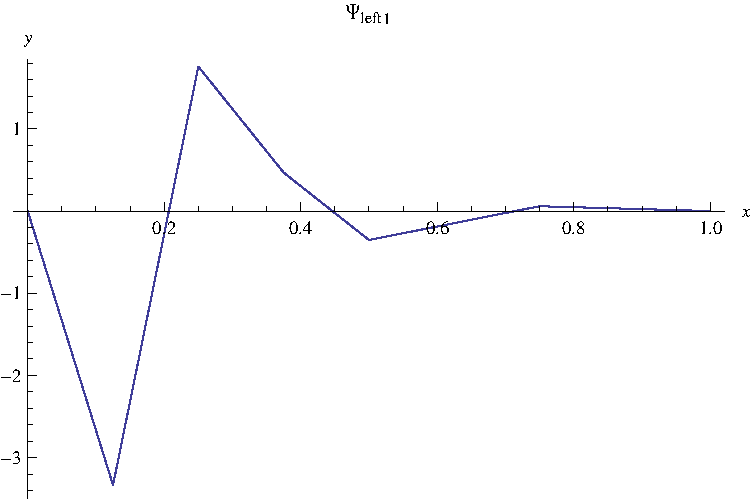
\includegraphics[width=20.cm]{linear_wavelet_dleft_1.pdf}\end{tabular} 
 \\ 
\begin{tabular}{c}
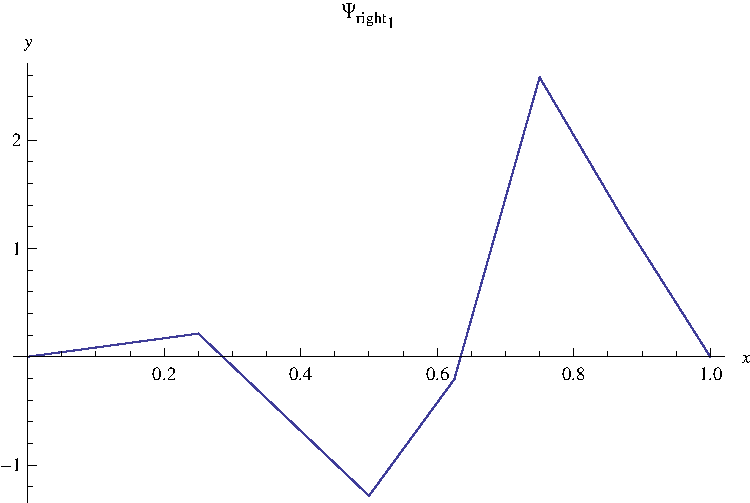
\includegraphics[width=20.cm]{linear_wavelet_dright_1.pdf}\end{tabular} 
 \end{landscape}
 \begin{landscape}
 \subsection{Validation}$$ \begin{array}{l|l}
\int_{-1}^1 f_1(x)f_2(x) dx& \Psi_{\text{left},1}(x) \\ \hline 
 \Psi_{\text{left},1}(x) & 1.0000 \\ 
\end{array} $$
$$ \begin{array}{l|lll}
\int_{-1}^1 f_1(x)f_2(x) dx& \varphi_1(x)& \varphi_2(x)& \varphi_3(x) \\ \hline 
 \Psi_{\text{left},1}(x) & 0.\cdot 10^{(-91)} & 0.\cdot 10^{(-90)} & -0.41248 \\ 
\end{array} $$ 
$$ \begin{array}{l|lll}
\int_{-1}^1 f_1(x)f_2(x) dx& \varphi_1(x-1)& \varphi_2(x-1)& \varphi_3(x-1) \\ \hline 
 \Psi_{\text{left},1}(x) & 0 & 0 & 0.\cdot 10^{(-91)} \\ 
\end{array} $$ 
$$ \begin{array}{l|lll}
\int_{-1}^1 f_1(x)f_2(x) dx& \Psi_1(x)& \Psi_2(x)& \Psi_3(x) \\ \hline 
 \Psi_{\text{left},1}(x) & 0.\cdot 10^{(-90)} & -0.81223 & 0.41248 \\ 
\end{array} $$ 
$$ \begin{array}{l|lll}
\int_{-1}^1 f_1(x)f_2(x) dx& \Psi_1(x-1)& \Psi_2(x-1)& \Psi_3(x-1) \\ \hline 
 \Psi_{\text{left},1}(x) & 0 & 0.\cdot 10^{(-90)} & 0.\cdot 10^{(-90)} \\ 
\end{array} $$ 
$$ \begin{array}{l|l}
\int_{-1}^1 f_1(x)f_2(x) dx& \Psi_{\text{right},1}(x) \\ \hline 
 \Psi_{\text{right},1}(x) & 1.0000 \\ 
\end{array} $$
$$ \begin{array}{l|lll}
\int_{-1}^1 f_1(x)f_2(x) dx& \varphi_1(x)& \varphi_2(x)& \varphi_3(x) \\ \hline 
 \Psi_{\text{right},1}(x) & 0.\cdot 10^{(-60)} & 0.\cdot 10^{(-60)} & 0.\cdot 10^{(-61)} \\ 
\end{array} $$ 
$$ \begin{array}{l|lll}
\int_{-1}^1 f_1(x)f_2(x) dx& \varphi_1(x-1)& \varphi_2(x-1)& \varphi_3(x-1) \\ \hline 
 \Psi_{\text{right},1}(x) & 0 & 0 & 0.57433 \\ 
\end{array} $$ 
$$ \begin{array}{l|lll}
\int_{-1}^1 f_1(x)f_2(x) dx& \Psi_1(x)& \Psi_2(x)& \Psi_3(x) \\ \hline 
 \Psi_{\text{left},1}(x) & 0.\cdot 10^{(-59)} & 0.\cdot 10^{(-61)} & 0.\cdot 10^{(-61)} \\ 
\end{array} $$ 
$$ \begin{array}{l|lll}
\int_{-1}^1 f_1(x)f_2(x) dx& \Psi_1(x-1)& \Psi_2(x-1)& \Psi_3(x-1) \\ \hline 
 \Psi_{\text{left},1}(x) & 0 & -0.58334 & -0.57433 \\ 
\end{array} $$ 
$$ \begin{array}{l|l}
\int_{-1}^1 f_1(x)f_2(x) dx& \Psi_{\text{left},1}(x) \\ \hline 
 \Psi_{\text{right},1}(x) & 0.\cdot 10^{(-61)} \\ 
\end{array} $$ 
\end{landscape}
\end{document}

